
\documentclass[aspectratio=1610,xcolor=dvipsnames]{beamer}
\usetheme[sectionslides]{SimplePlusNord}

\usepackage{graphicx}

\title{SimplePlusNord-BeamerTheme}
\subtitle{A Beamer theme in the Nord colours}

\author{Name Surname}

\institute{Organization}
\date{\today}
\titlegraphic{\scriptsize Nord colours: nordtheme.com, MIT licence}

\begin{document}

\begin{frame}
    \titlepage
\end{frame}

\section{Text elements}

\subsection{Overview}
% Steps on the left, the overview they produce on the right ([fragile] because of the code boxes)
\begin{frame}[fragile]{Overview}
\begin{columns}[T,onlytextwidth]
\begin{column}{0.5\textwidth}
\textbf{1. Choose when it appears}\par\smallskip
\begin{codeonly}
\usetheme[sectionslides]
   {SimplePlusNord}
\end{codeonly}
\smallskip
\textbf{2. List the slides}\par\smallskip
\begin{codeonly}
\subsection{Title}
\end{codeonly}
\smallskip
\textbf{3. Optional}\par\smallskip
\begin{codeonly}
\tocnumbers
\end{codeonly}
\end{column}
\begin{column}{0.45\textwidth}
\tableofcontents[currentsection,subsectionstyle=show/show/hide]
\end{column}
\end{columns}
\end{frame}

\subsection{Bullet Points}
\begin{frame}{Bullet Points}
    \begin{itemize}
        \item A short point
        \item A second point, a little longer than the first
        \item A third point, long enough to wrap onto a second line, so that the hanging indent of the list shows
        \item A fourth point
        \item A fifth point, with nothing more to say
        \item \fade{Faded with \texttt{\textbackslash fade}, \textcolor{nord10}{and the blue inside is lightened too}}
    \end{itemize}
\end{frame}

\subsection{Boxes of Highlighted Text}
\begin{frame}{Boxes of Highlighted Text}
    A few words can stand out in \alert{bold}; use it sparingly.

    \begin{infobox}{Box}
        Sample text
    \end{infobox}

    \begin{alertbox}{Alertbox}
        Sample text in a box that warns
    \end{alertbox}

    \begin{examplebox}{Examplebox}
        Sample text in a box that illustrates
    \end{examplebox}
\end{frame}

\subsection{Boxes: code}
% Steps with their code on the left, the result on the right
\begin{frame}[fragile]{Boxes: code and result}
\begin{columns}[T,onlytextwidth]
\begin{column}{0.5\textwidth}
\textbf{1. A box}\par\smallskip
\begin{codeonly}
\begin{infobox}{Title}
  Text
\end{infobox}
\end{codeonly}
\smallskip
\textbf{2. Alert and example}\par\smallskip
\begin{codeonly}
\begin{alertbox}{Title}
\begin{examplebox}{Title}
\end{codeonly}
\end{column}
\begin{column}{0.45\textwidth}
\begin{infobox}{Box}
    Sample text
\end{infobox}
\begin{alertbox}{Alertbox}
    Sample text
\end{alertbox}
\begin{examplebox}{Examplebox}
    Sample text
\end{examplebox}
\end{column}
\end{columns}
\end{frame}

% codedoc: to print the line \end{codeonly} inside a code box, that box needs a different name
\newtcblisting{codedoc}{splusnord code,listing only}

\subsection{Code boxes}
\begin{frame}[fragile]{Code boxes}
\begin{columns}[T,onlytextwidth]
\begin{column}{0.5\textwidth}
\textbf{1. Make the frame fragile}\par\smallskip
\begin{codedoc}
\begin{frame}[fragile]{Title}
\end{codedoc}
\smallskip
\textbf{2. Code only}\par\smallskip
\begin{codedoc}
\begin{codeonly}
  \alert{some code}
\end{codeonly}
\end{codedoc}
\smallskip
\textbf{3. Code and result}\par\smallskip
\begin{codedoc}
\begin{codeexample}
  \textbf{bold}
\end{codeexample}
\end{codedoc}
\end{column}
\begin{column}{0.45\textwidth}
\begin{codeonly}
\alert{some code}
\end{codeonly}
\begin{codeexample}
\textbf{bold}
\end{codeexample}
\end{column}
\end{columns}
\end{frame}

\subsection{Multiple Columns}
\begin{frame}{Multiple Columns}
    \begin{columns}[c]
        \column{.45\textwidth}
        \textbf{Steps}
        \begin{enumerate}
            \item State the claim
            \item Explain it
            \item Give an example
        \end{enumerate}

        \column{.45\textwidth}
        Columns split the slide in parts of the width you choose, and each part flows as its own text, as in a newspaper. They are centred vertically here; \texttt{[T]} aligns them on their first line.
    \end{columns}
\end{frame}

\section{Data and references}

\subsection{Table}
\begin{frame}{Table}
    \begin{table}
        \begin{tabular}{l r r}
            \textbf{Group} & \textbf{Mean} & \textbf{Deviation} \\
            \headrule
            Control             & 0.562               & 0.0123              \\ \hline
            Low dose            & 0.910               & 0.0456              \\ \hline
            High dose           & 0.296               & 0.0089              \\
        \end{tabular}
        \caption{Three groups of the experiment}
    \end{table}
    \source{Verdi (2021), Table 2}
\end{frame}

\subsection{Table: code}
\begin{frame}[fragile]{Table: code and result}
\begin{columns}[T,onlytextwidth]
\begin{column}{0.5\textwidth}
\textbf{1. Header and rule}\par\smallskip
\begin{codeonly}
\textbf{Group} & \textbf{Mean} \\
\headrule
\end{codeonly}
\smallskip
\textbf{2. Rows}\par\smallskip
\begin{codeonly}
Control & 0.562 \\ \hline
Treated & 0.910 \\
\end{codeonly}
\smallskip
\textbf{3. Source}\par\smallskip
\begin{codeonly}
\source{Verdi (2021)}
\end{codeonly}
\end{column}
\begin{column}{0.45\textwidth}
\begin{table}
  \begin{tabular}{l r}
    \textbf{Group} & \textbf{Mean} \\
    \headrule
    Control & 0.562 \\ \hline
    Treated & 0.910 \\
  \end{tabular}
  \caption{Group means}
\end{table}
\source{Verdi (2021)}
\end{column}
\end{columns}
\end{frame}

\subsection{Theorem}
\begin{frame}{Theorem}
    \begin{theorem}[Pythagoras]
        $a^{2}+b^{2}=c^{2}$
    \end{theorem}

    \begin{theorem}[A formula for the stress test]
        \[
            \mathcal{F}[f](\xi)=\int_{-\infty}^{\infty} f(x)\,e^{-2\pi i x\xi}\,dx,\qquad
            \zeta(s)=\sum_{n=1}^{\infty}\frac{1}{n^{s}}=\prod_{p\ \mathrm{prime}}\frac{1}{1-p^{-s}}
        \]
        \[
            \hat{\boldsymbol\beta}=\bigl(\mathbf{X}^{\top}\mathbf{X}\bigr)^{-1}\mathbf{X}^{\top}\mathbf{y},\quad
            \mathbf{A}=\begin{pmatrix}a_{11}&\cdots&a_{1n}\\\vdots&\ddots&\vdots\\a_{m1}&\cdots&a_{mn}\end{pmatrix},\quad
            \binom{n}{k}=\frac{n!}{k!\,(n-k)!}
        \]
        \[
            \lim_{n\to\infty}\Pr\!\Bigl(\frac{\bar{X}_n-\mu}{\sigma/\sqrt{n}}\le z\Bigr)
            =\frac{1}{\sqrt{2\pi}}\int_{-\infty}^{z}e^{-t^{2}/2}\,dt=\Phi(z)
        \]
    \end{theorem}
\end{frame}

\subsection{Definitions and examples}
\begin{frame}[fragile]{Definitions and examples}
\begin{columns}[T,onlytextwidth]
\begin{column}{0.5\textwidth}
\textbf{1. A definition}\par\smallskip
\begin{codeonly}
\begin{definition}[Title]
  Text with \alert{emphasis}
\end{definition}
\end{codeonly}
\smallskip
\textbf{2. An example}\par\smallskip
\begin{codeonly}
\begin{example}
  Text
\end{example}
\end{codeonly}
\end{column}
\begin{column}{0.45\textwidth}
\begin{definition}[Estimator]
    A rule that turns a sample into a guess is an \alert{estimator}.
\end{definition}
\begin{example}
    The sample mean $\bar{x}$ estimates $\mu$.
\end{example}
\end{column}
\end{columns}
\end{frame}

\subsection{Theorems and proofs}
\begin{frame}[fragile]{Theorems and proofs}
\begin{columns}[T,onlytextwidth]
\begin{column}{0.5\textwidth}
\textbf{1. A lemma, with its proof}\par\smallskip
\begin{codeonly}
\begin{lemma}
  Statement
  \begin{proof}
    Proof text
  \end{proof}
\end{lemma}
\end{codeonly}
\smallskip
\textbf{2. A theorem or a corollary}\par\smallskip
\begin{codeonly}
\begin{theorem}[Title]
\begin{corollary}
\end{codeonly}
\end{column}
\begin{column}{0.45\textwidth}
\begin{lemma}
    $\operatorname{Var}(aX)=a^{2}\operatorname{Var}(X)$.
    \begin{proof}
        Expand and take $a^{2}$ out.
    \end{proof}
\end{lemma}
\begin{theorem}[Pythagoras]
    $a^{2}+b^{2}=c^{2}$.
\end{theorem}
\end{column}
\end{columns}
\end{frame}

\subsection{Formulas: code}
\begin{frame}[fragile]{Formulas: code and result}
\begin{columns}[T,onlytextwidth]
\begin{column}{0.5\textwidth}
\textbf{1. A theorem}\par\smallskip
\begin{codeonly}
\begin{theorem}[Title]
  $\bar{X}_n \xrightarrow{p} \mu$
\end{theorem}
\end{codeonly}
\smallskip
\textbf{2. A formula}\par\smallskip
\begin{codeonly}
\[
  t=\frac{\bar{x}-\mu_0}{s/\sqrt{n}}
\]
\end{codeonly}
\end{column}
\begin{column}{0.45\textwidth}
\begin{theorem}[Large numbers]
    $\bar{X}_n \xrightarrow{p} \mu$
\end{theorem}
\[
  t=\frac{\bar{x}-\mu_0}{s/\sqrt{n}}
\]
\end{column}
\end{columns}
\end{frame}

\subsection{Figure: transparent}
\begin{frame}[fragile]{Figure: transparent}
\begin{columns}[T,onlytextwidth]
\begin{column}{0.5\textwidth}
\textbf{1. A figure with alpha}\par\smallskip
\begin{codeonly}
\begin{figure}
  \includegraphics[height=4cm]
    {graph.png}
  \caption{Caption}
\end{figure}
\end{codeonly}
\smallskip
\textbf{2. Name the source}\par\smallskip
\begin{codeonly}
\source{AVDLCZ, CC0}
\end{codeonly}
\end{column}
\begin{column}{0.45\textwidth}
\begin{figure}
    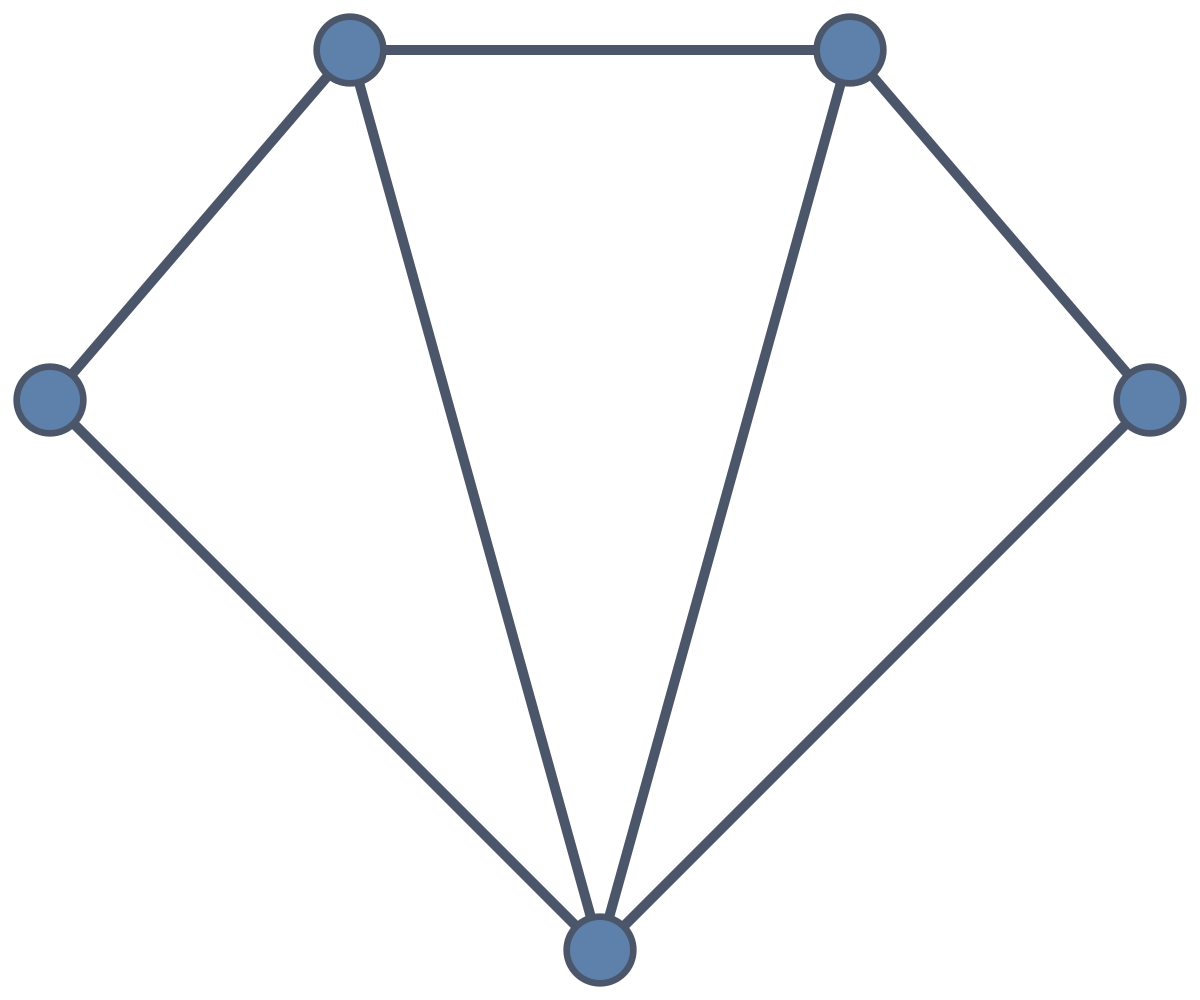
\includegraphics[height=0.5\textheight]{images/graph.png}
    \caption{A PNG with a transparent background sits on the slide as it is}
\end{figure}
\source{AVDLCZ, CC0}
\end{column}
\end{columns}
\end{frame}

\subsection{Figure: opaque}
\begin{frame}[fragile]{Figure: opaque}
\begin{columns}[T,onlytextwidth]
\begin{column}{0.5\textwidth}
\textbf{1. A photo, corners rounded}\par\smallskip
\begin{codeonly}
\begin{figure}
  \roundedgraphics
    [height=4cm]{photo.jpg}
  \caption{Caption}
\end{figure}
\end{codeonly}
\smallskip
\textbf{2. Name the source}\par\smallskip
\begin{codeonly}
\source{NASA / B. Anders}
\end{codeonly}
\end{column}
\begin{column}{0.45\textwidth}
\begin{figure}
    \roundedgraphics[height=0.5\textheight]{images/earthrise.jpg}
    \caption{A photo keeps its own background, with the corners slightly rounded}
\end{figure}
\source{NASA / B. Anders}
\end{column}
\end{columns}
\end{frame}

\subsection{Citation}
\begin{frame}[fragile]{Citation}
    \verb|\cite| gives the number of the entry in the list of references.

    One work is cited like this \cite{p1}, two at once like this \cite{p1,p2}.
\end{frame}

\subsection{Citation: code}
\begin{frame}[fragile]{Citation: code and result}
\begin{columns}[T,onlytextwidth]
\begin{column}{0.5\textwidth}
\textbf{1. Cite}\par\smallskip
\begin{codeonly}
\cite{p1}
\cite{p1,p2}
\end{codeonly}
\smallskip
\textbf{2. Name the sources}\par\smallskip
\begin{codeonly}
\source{Verdi (2021)}
\source{Rossi (2019)}
\end{codeonly}
\smallskip
\textbf{3. Lighten a remark}\par\smallskip
\begin{codeonly}
\fade{remark}
\end{codeonly}
\end{column}
\begin{column}{0.45\textwidth}
One source \cite{p1}, two at once \cite{p1,p2}, and a faded \fade{remark}.
\source{Verdi (2021)}\source{Rossi (2019)}
\end{column}
\end{columns}
\end{frame}

\subsection{References}
\begin{frame}{References}
    \footnotesize
    \bibliographystyle{unsrt}% numeric, in order of first citation
    \bibliography{reference}
\end{frame}

\subsection{Questions}
% \darkslide, put right after \begin{frame}, turns any slide dark like the first one
\begin{frame}{Questions}
    \darkslide
    {\Huge\bfseries Thank you}\par\bigskip
    {\Large Questions?}
\end{frame}

\end{document}